
\documentclass[11pt]{article}
\usepackage{graphicx}
\usepackage[includeheadfoot,
            left=1in,
            right=1in,
            top=1cm,
            bottom=1cm,
            headheight=1cm]{geometry} % geometry needs to know headheight to correctly render the footer
\usepackage{multirow}
\usepackage{adjustbox}
\usepackage{hyperref}
\usepackage{wrapfig}
\usepackage{subfigure}


\hypersetup{
    colorlinks=true,
    linkcolor=blue,
    filecolor=magenta,      
    urlcolor=cyan,
    pdftitle={Overleaf Example},
    pdfpagemode=FullScreen,
    }
	

\title{PROGETTO OBJECT ORIENTATION\\Corso di laurea in Informatica\\Insegnamento Object Orientation
\\ Professore Tramontana Porfirio \\ANNO ACCADEMICO 2022/2023  }
\author{Studente Adolfo Torcicollo N86003538}
\date{13 gennaio 2023}

%per modificare font scrivere questo comando \sffamily e per rimuoverlo \rmsffamily sffamily è un esempio di font

\begin{document}

	\begin{figure}
		\centering
		
\includegraphics[width=0.8\linewidth]{UNINA-2.jpg}
		\maketitle
	\end{figure}


	\clearpage

	\part{Descrizione del progetto}
	\section{Traccia del Progetto}

	Si sviluppi un sistema informativo, composto da una base di dati relazionale e da un applicativo Java dotato di GUI (Swing o 
	Java FX), per la gestione delle librerie musicali di un gruppo di utenti. Di ogni traccia si deve gestire l’album di appartenenza 
	(ogni traccia ha un solo album di appartenenza – remastering diversi della stessa traccia possono far parte di album diversi), 
	l’artista e la versione (l’anno). Ogni utente è identificato da un nome utente, univoco in tutto il sistema. Una traccia è 
	identificata dall’album di appartenenza, dall’autore e dall’anno. Modellare il concetto di cover, secondo il quale, una traccia 
	“nasce” in un determinato anno e un artista ne effettua una personale rivisitazione. Il concetto di cover è diverso dal concetto
	di remastering: la cover è una traccia eseguita da un altro artista, il remastering è la stessa traccia le cui equalizzazioni vengono 
	modificate utilizzando tecnologie diverse. Il sistema permette ad un admin di recuperare, data una certa traccia, un 
	sottoinsieme degli utenti che hanno effettuato più ascolti di quella traccia, andando a differenziare la versione per cui è stata 
	ascoltata la traccia. Deve essere inoltre possibile andare a identificare la fascia oraria in cui un determinato utente ha 
	effettuato più ascolti (definire un set di fasce orarie, per semplificarne il compito).

	\section{Analisi Del Problema}
	Bisogna gestire i dati con l'utilizzo di classi, quindi si è stato deciso di scegliere cinque classi aiuteranno la gestione dei dati per
	l'applicativo.
	\\
	\\
	\\
	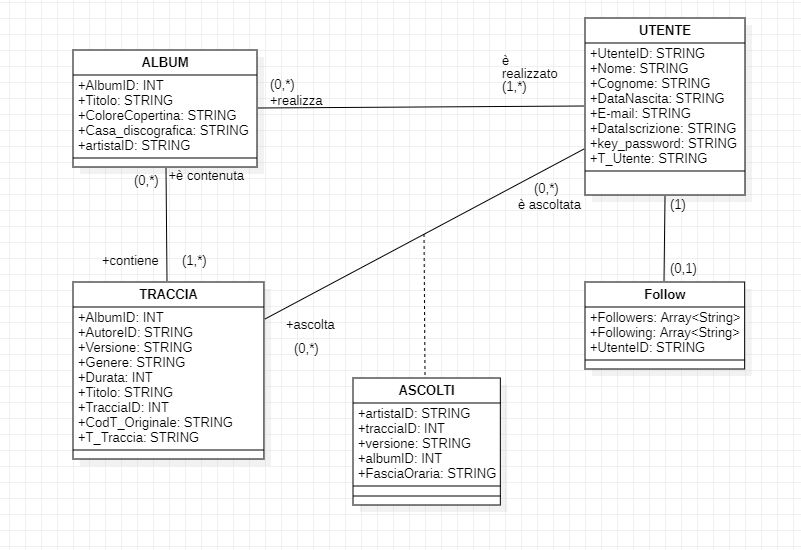
\includegraphics[width=0.8\linewidth]{Dominio del Problema.png} \footnote{link : \href{https://github.com/torcy-it/PROGETTO-BD-OO}{Class diagram nel dominio del Problema}}




	\clearpage
	
	\section{Soluzione del Problema}
	A fronte di un’analisi, è stato scelto di gestire la piattaforma che fa uso di una database che consente una gestione persistente dei dati essendo anch'esso ,concettualmente, un file. 
	Il database scelto è stato collegato all'applicativo tramite un approccio che utilizza classi presenti nel package DAO.Ogni classeDAO viene inizializzata tramite la classe chiamata ConnessioneDAO 
	che a sua volta è la sola ad avere accesso alla classe che ha accesso alla connessione del database. Il nome di tale classe è DatabasePg che avvia la connessione al database.
	Le classi del packageDAO verranno inizializzate dal controller un oggetto che trasporta tra una gui e l'altra il carico utile per l'utilizzo di funzioni nell'applicativo come il cambio di finestra.
	Il controller verrà inizializzato dalla prima finestra di visualizzazione dell'applicativo cioè la LoginWindow. I controllerFXML sono necessari rer poter vedere in azione l'interfaccia creata dai fileFXML.
	\\
	\\
	\\
	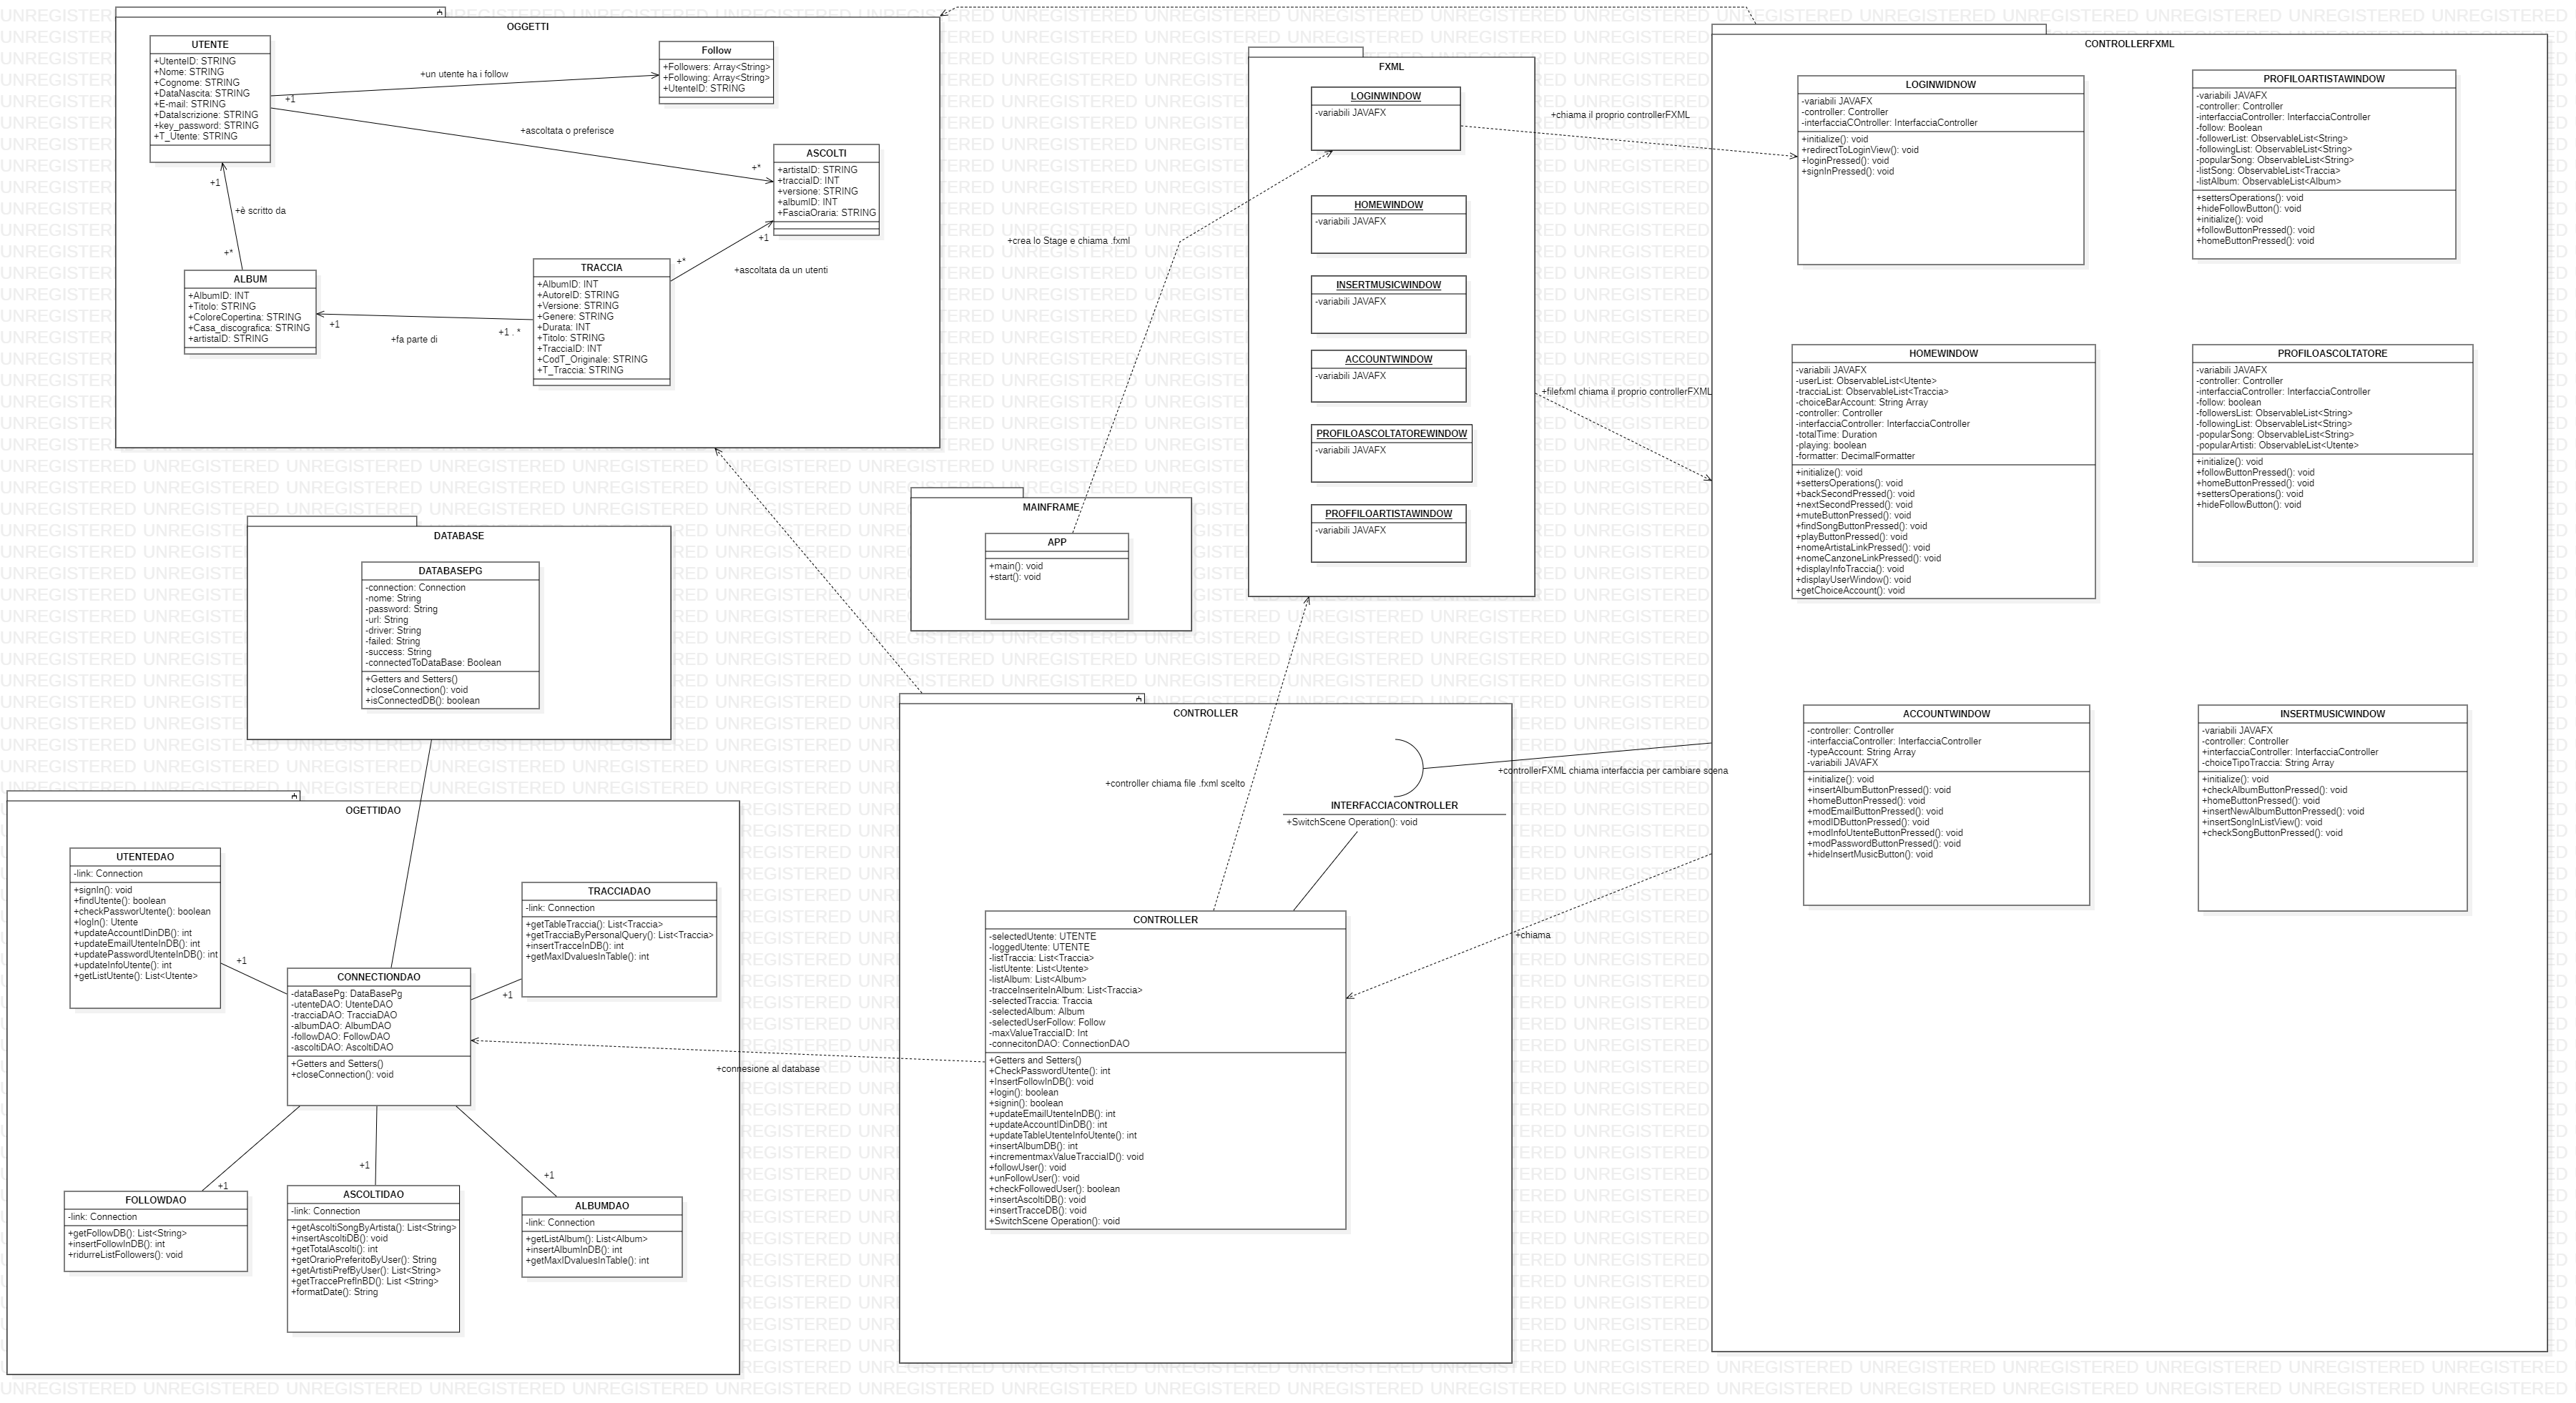
\includegraphics[width=1\linewidth]{dominio Della soluzione.png} \footnote{link : \href{https://github.com/torcy-it/PROGETTO-BD-OO}{Class diagram nel dominio della Soluzione}}
	
	\clearpage
	\section{Sequence Diagrams}
	\subsection{Sequence Diagram per il Login}
	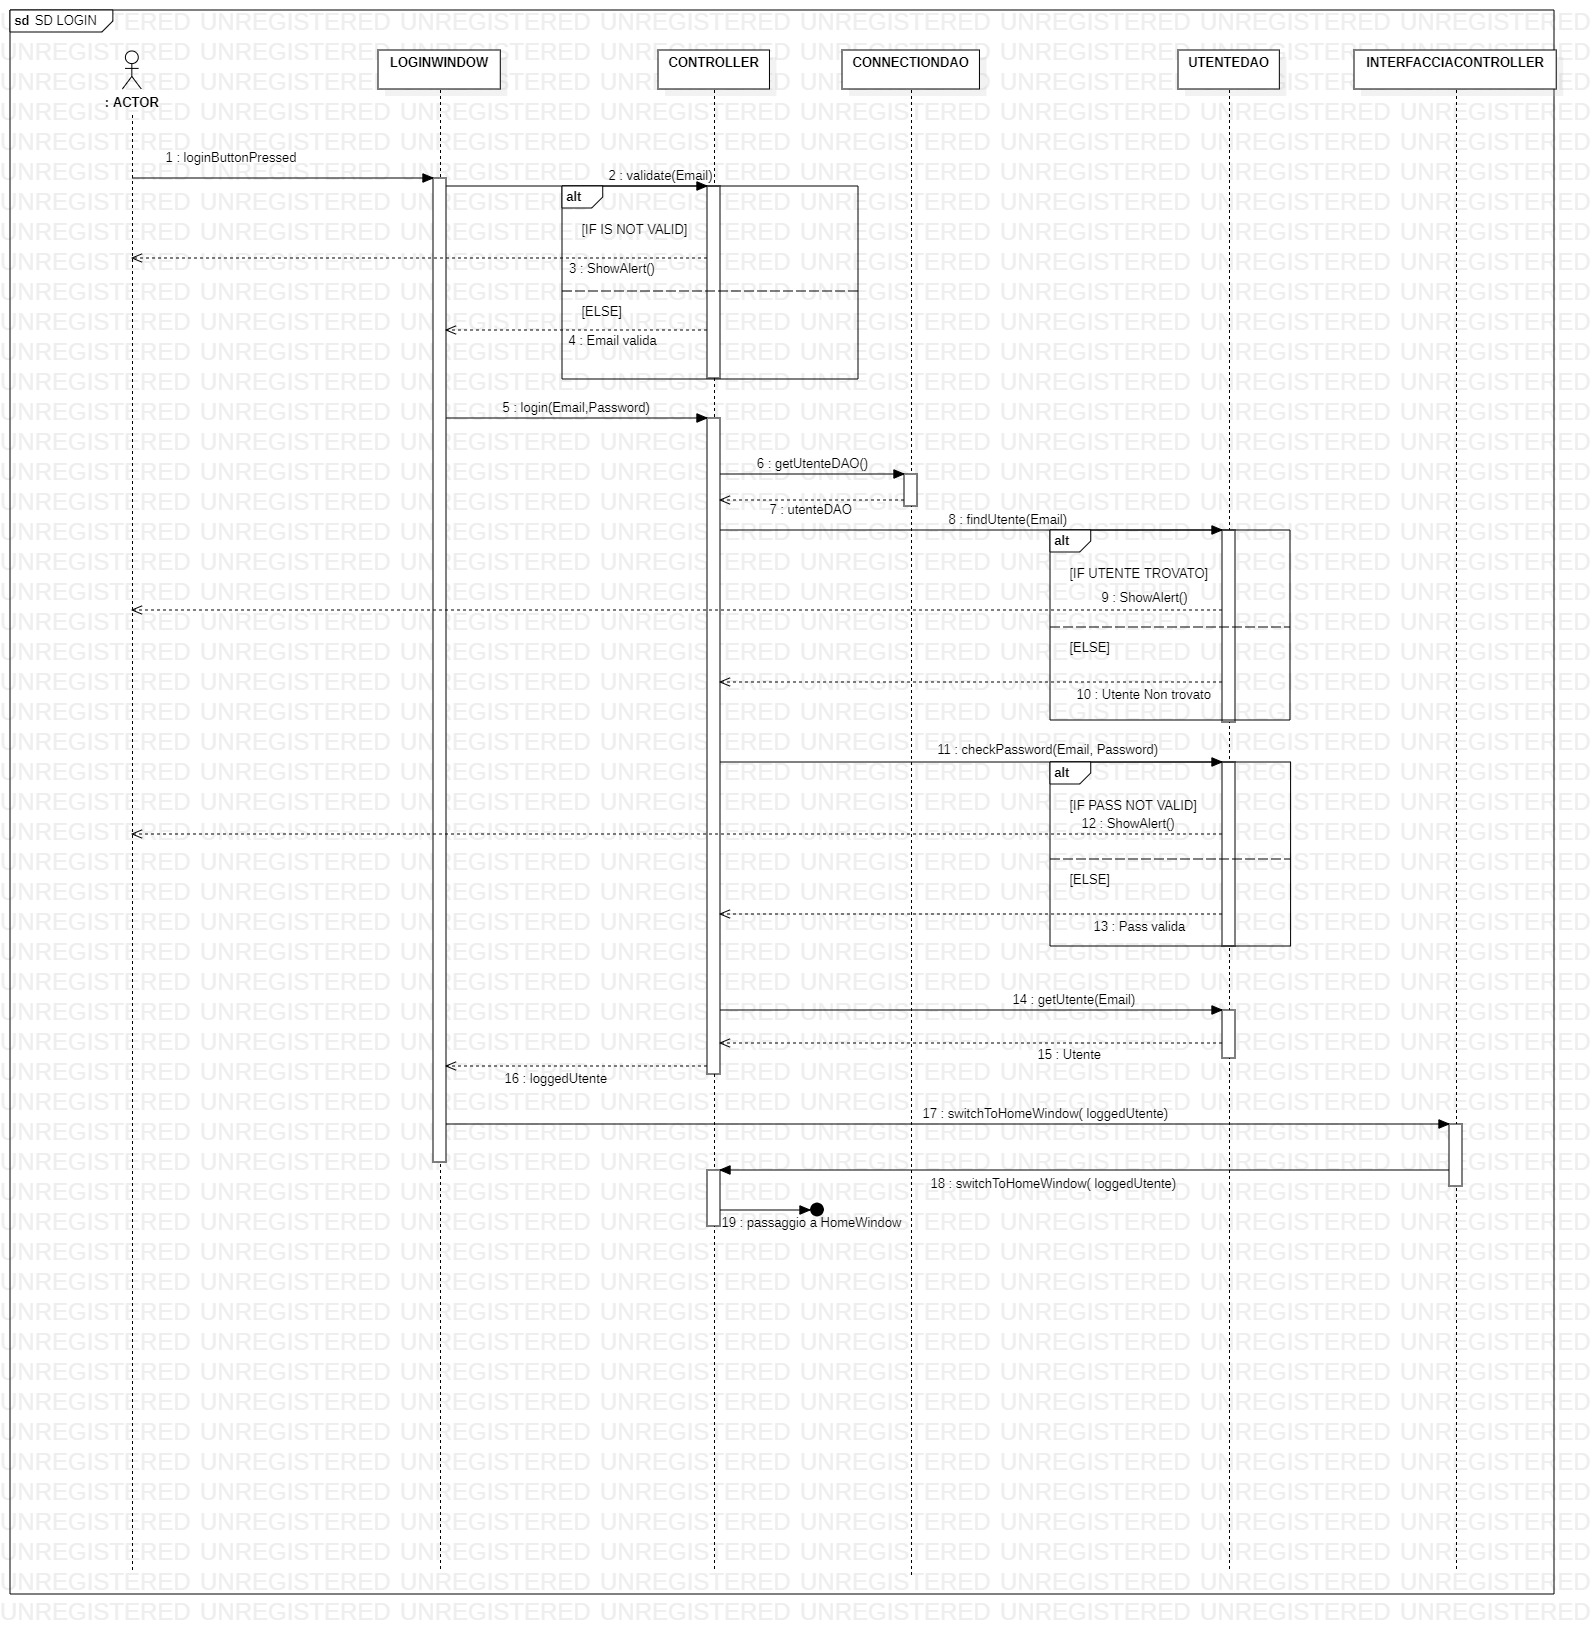
\includegraphics[width=1.1\linewidth]{SD LOGIN.jpg} \footnote{link : \href{https://github.com/torcy-it/LettoreMusicale/tree/main/DocumentazioneProgetto/SequenceDiagrams}{Sequence Diagram Login}}
	\clearpage
	\subsection{Sequence Diagram Follow User}
	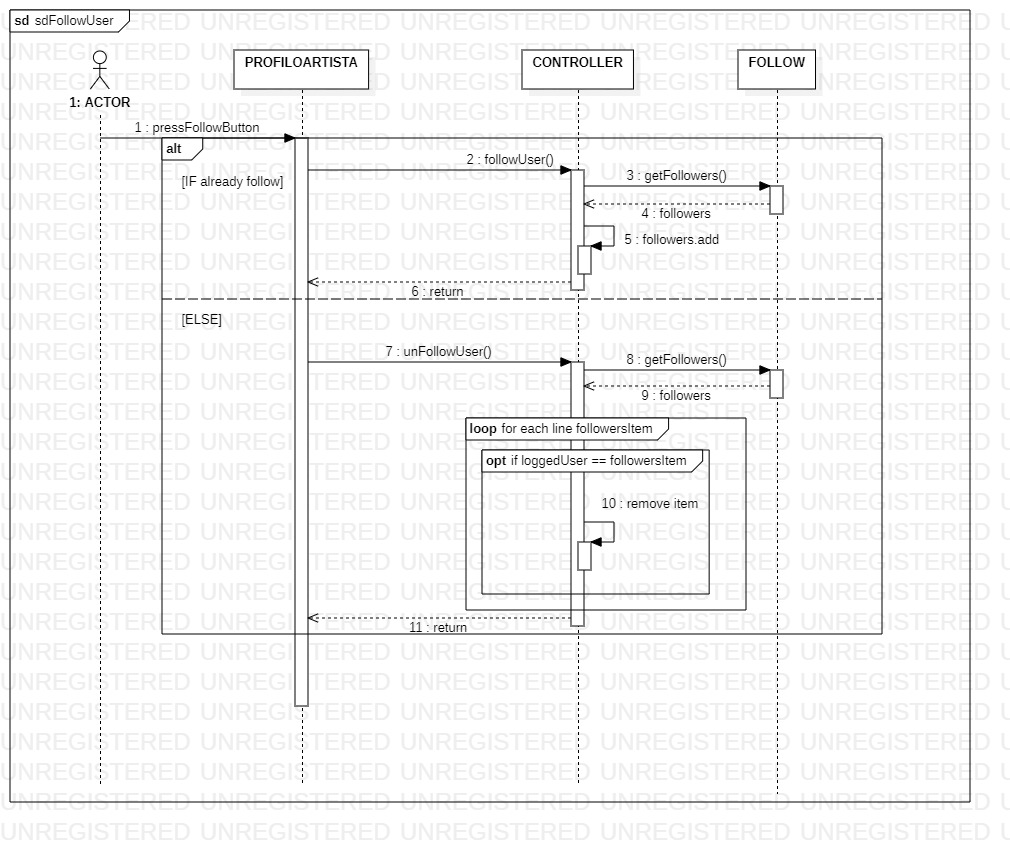
\includegraphics[width=1.2\linewidth]{sdFollowUser.jpg} \footnote{link : \href{https://github.com/torcy-it/LettoreMusicale/tree/main/DocumentazioneProgetto/SequenceDiagrams}{Sequence Diagram Follow User}}
	
	\clearpage
	\section{CRC CARDS}
	

	\subsection{Oggetto DataBasePg}

	\begin{table}[h]
		\centering
		\begin{adjustbox}{max width=\textwidth}
			\begin{tabular}{|l|l|l|} \hline
			CLASSE  & RESPONSABILITA'                                                                                                                                                                                        & COLLABORATORE                                                                                                                                                                                                                                                                                                                                                                                                                                                                                                                                                                                                                                              \\\hline
			\hline
			DATABASEPG   & \begin{tabular}[c]{@{}l@{}}\textbullet Crea e chiude la connessione con il database Postgres\\\end{tabular} 															& \begin{tabular}[c]{@{}l@{}} \end{tabular}                                                                                                                                                                                                                              \\\hline                                                                                                                                                                                                                                                                                                                                                                                
			\end{tabular}
		\end{adjustbox}
	\end{table}


	\subsection{OggettiDAO}

	\begin{table}[h]
		\centering
		\begin{adjustbox}{max width=\textwidth}
			\begin{tabular}{|l|l|l|} \hline
			CLASSE  & RESPONSABILITA'                                                                                                                                                                                        & COLLABORATORE                                                                                                                                                                                                                                                                                                                                                                                                                                                                                                                                                                                                                                              \\\hline
			\hline
			CONNECTIONDAO   & \begin{tabular}[c]{@{}l@{}}\textbullet Inizializza l'ogetto DatabasePg che crea una conessione \\al database e con tale connessione inizializza gli \\ogettiDAO\\\end{tabular} 															& \begin{tabular}[c]{@{}l@{}}\textopenbullet DataBasePg \\\textopenbullet AlbumDAO\\\textopenbullet TracciaDAO \\\textopenbullet AscoltiDAO\\ \textopenbullet FollowDAO \\\textopenbullet  UtenteDAO \end{tabular}                                                                                                                                                                                                                              \\\hline
			\hline
			ALBUMDAO & \begin{tabular}[c]{@{}l@{}}\textbullet Inserisce Albums nel Database \\\textbullet Preleva Albums nel database \\\end{tabular}              						& \begin{tabular}[c]{@{}l@{}}      \end{tabular} \\\hline
			\hline
			UTENTEDAO  & \begin{tabular}[c]{@{}l@{}}\textbullet Aggiorna valori Utente nel database\\\textbullet Inserisce utente nel database \\\textbullet Preleva Utente nel database\end{tabular}                                                                                             & \begin{tabular}[c]{@{}l@{}}\textopenbullet Utente       \end{tabular}                                                                                                                                                                   \\\hline
			\hline
			ASCOLTIDAO     & \begin{tabular}[c]{@{}l@{}}\textbullet Inserisce Ascolti nel Database \\\textbullet Preleva AscoltiTracce nel database\\\textbullet Preleva AscoltiOrario nel database \\\textbullet Preleva AscoltiArtisti nel database   \end{tabular}                                                    & \begin{tabular}[c]{@{}l@{}}\textopenbullet Utente\\ \textopenbullet Traccia \\\textopenbullet Ascolti       \end{tabular}                                                                                                                                                                                                                                                                                                                                                                                             \\ \hline
			\hline
			FOLLOWDAO     & \begin{tabular}[c]{@{}l@{}}\textbullet Inserisce Follow nel Database \\\textbullet Preleva Follow nel database  \end{tabular}                                                    & \begin{tabular}[c]{@{}l@{}} \textopenbullet Follow      \end{tabular}                                                                                                                                                                                                                                                                                                                                                                                             \\ \hline
			\hline
			TRACCIADAO     & \begin{tabular}[c]{@{}l@{}}\textbullet Inserisce Traccia nel Database \\\textbullet Preleva Traccia nel database  \end{tabular}                                                    & \begin{tabular}[c]{@{}l@{}} \textopenbullet Traccia      \end{tabular}                                                                                                                                                                                                                                                                                                                                                                                             \\ \hline
			\end{tabular}
		\end{adjustbox}
	\end{table}

	\clearpage
	\subsection{ControllerFXML}

	\begin{table}[h]
		\centering
		\begin{adjustbox}{max width=\textwidth}
			\begin{tabular}{|l|l|l|} \hline
			CLASSE  & RESPONSABILITA'                                                                                                                                                                                        & COLLABORATORE                                                                                                                                                                                                                                                                                                                                                                                                                                                                                                                                                                                                                                              \\\hline
			\hline
			ACCOUNTWINDOW   & \begin{tabular}[c]{@{}l@{}}\textbullet Form per la modifica di informazioni\\ personali dell'utente\\\textbullet Permette di cambiare scena in \\InserMusicWindow\\\textbullet Permette di cambiare scena in \\HomeWindow\end{tabular} 															& \begin{tabular}[c]{@{}l@{}}\textopenbullet Controller \\ \textopenbullet InterfacciaController\end{tabular}                                                                                                                                                                                                                              \\\hline
			\hline
			HOMEWINDOW & \begin{tabular}[c]{@{}l@{}}\textbullet Cercare tracce/utenti/Artisti \\\textbullet Permette di cambiare scena in \\ProfiloArtista o Ascoltatore\\\textbullet Permette di scegliere il minutaggio\\ di una traccia\\\textbullet Permette di cambiare scena in AccountWindow\\\textbullet Permette di Ascoltare una Traccia \\\textbullet Permette di cercare le tracce appartenenti\\ ad un determinato album\\\end{tabular}              						& \begin{tabular}[c]{@{}l@{}}     \textopenbullet Controller \\ \textopenbullet InterfacciaController \end{tabular} \\\hline
			\hline
			INSERTMUSICWINDOW  & \begin{tabular}[c]{@{}l@{}}\textbullet Form per l'inserimento di album e Tracce\\\textbullet Permette di cambiare scena in \\HomeWindow \end{tabular}                                                                                             & \begin{tabular}[c]{@{}l@{}}\textopenbullet Controller\\ \textopenbullet InterfacciaController       \end{tabular}                                                                                                                                                                   \\\hline
			\hline
			LOGINWINDOW     & \begin{tabular}[c]{@{}l@{}}\textbullet Form per il Login e Signin \end{tabular}                                                    & \begin{tabular}[c]{@{}l@{}}\textopenbullet Controller\\ \textopenbullet InterfacciaController      \end{tabular}                                                                                                                                                                                                                                                                                                                                                                                             \\ \hline
			\hline
			PROFILOARTISTAWINDOW     & \begin{tabular}[c]{@{}l@{}}\textbullet Visualizza Informazioni relative alle \\ tracce popolari e discografia e infine\\ i followers e following \\\textbullet Permette di cambiare scena in \\HomeWindow \\\textbullet Permette di togliere il segui/seguire l'artista    \end{tabular}                                                    & \begin{tabular}[c]{@{}l@{}} \textopenbullet Controller\\ \textopenbullet InterfacciaController      \end{tabular}                                                                                                                                                                                                                                                                                                                                                                                             \\ \hline
			\hline
			PROFILOASCOLTATOREWINDOW     & \begin{tabular}[c]{@{}l@{}}\textbullet Visualizza Informazioni relative alle \\ tracce  e aritisti preferiti e infine\\ i followers e following \\\textbullet Permette di cambiare scena in \\HomeWindow \\\textbullet Permette di togliere il segui/seguire l'utente    \end{tabular}                                                    & \begin{tabular}[c]{@{}l@{}} \textopenbullet Controller \\\textopenbullet InterfacciaController   \end{tabular}                                                                                                                                                                                                                                                                                                                                                                                             \\ \hline
			\end{tabular}
		\end{adjustbox}
	\end{table}
	\clearpage
	\subsection{Model}

	\begin{table}[h]
		\centering
		\begin{adjustbox}{max width=\textwidth}
			\begin{tabular}{|l|l|l|} \hline
			CLASSE  & RESPONSABILITA'                                                                                                                                                                                        & COLLABORATORE                                                                                                                                                                                                                                                                                                                                                                                                                                                                                                                                                                                                                                              \\\hline
			\hline
			ALBUM   & \begin{tabular}[c]{@{}l@{}}\textbullet Contiene e fornisce informazioni riguardo un album e l'artista\\ che lo ha prodotto\end{tabular} 															& \begin{tabular}[c]{@{}l@{}}        \end{tabular}                                                                                                                                                                                                                              \\\hline
			\hline
			TRACCIA & \begin{tabular}[c]{@{}l@{}}\textbullet Contiene e fornisce informazioni riguardo una traccia di un album\\   di appartenenza e l'artista che lo ha prodotto\\\end{tabular}              						& \begin{tabular}[c]{@{}l@{}}        \end{tabular} \\\hline
			\hline
			UTENTE  & \begin{tabular}[c]{@{}l@{}}\textbullet Contiene e fornisce informazioni riguardo una traccia di un album\\   di appartenenza e l'artista che lo ha prodotto\end{tabular}                                                                                             & \begin{tabular}[c]{@{}l@{}}       \end{tabular}                                                                                                                                                                   \\\hline
			\hline
			ASCOLTI     & \begin{tabular}[c]{@{}l@{}}\textbullet Contiene e fornisce informazioni riguardo una traccia \\ con l'labum di appartenenza e l'artista includendo anche\\ il relativo ascoltatore\end{tabular}                                                    & \begin{tabular}[c]{@{}l@{}}       \end{tabular}                                                                                                                                                                                                                                                                                                                                                                                             \\ \hline
			\hline
			FOLLOW     & \begin{tabular}[c]{@{}l@{}}\textbullet Contiene e fornisce informazioni riguardo un utente\\ con i relativi followers e following\end{tabular}                                                    & \begin{tabular}[c]{@{}l@{}}       \end{tabular}                                                                                                                                                                                                                                                                                                                                                                                             \\ \hline
			\end{tabular}
		\end{adjustbox}
	\end{table}


	\subsection{Controller}

	\begin{table}[h]
		\centering
		\begin{adjustbox}{max width=\textwidth}
			\begin{tabular}{|l|l|l|} \hline
			CLASSE  & RESPONSABILITA'                                                                                                                                                                                        & COLLABORATORE                                                                                                                                                                                                                                                                                                                                                                                                                                                                                                                                                                                                                                              \\\hline
			\hline
			CONTROLLER   & \begin{tabular}[c]{@{}l@{}}\textbullet Si occupa della fase di Login di un Utente\\\textbullet Si occupa della fase di SignIn di un utente\\\textbullet Si occupa di operazioni relative al settaggio\\di liste Utente/Traccia/Album/Ascolti//Follow \\\textbullet Filtra le liste per una ricerca personale \\\textbullet Visualizza a schermo gli Allert\\\textbullet Imposta il LoggedUtente\\\textbullet Imposta un selectedUtente se selezionato  \\  \\\end{tabular} 															& \begin{tabular}[c]{@{}l@{}}\textopenbullet Traccia \\ \textopenbullet Follow \\ \textopenbullet Ascolti \\ \textopenbullet Album \\ \textopenbullet Utente \\ \textopenbullet ConnectionDAO \\\end{tabular}                                                                                                                                                                                                                              \\\hline                                                                                                                                                                                                                                                                                                                                                                                
			\hline
			INTERFACCIACONTROLLER     & \begin{tabular}[c]{@{}l@{}}\textbullet Cambia le Scene tramite una selezione personale\\ dell'untente\end{tabular}                                                    & \begin{tabular}[c]{@{}l@{}} \textopenbullet Controller      \end{tabular}                                                                                                                                                                                                                                                                                                                                                                                             \\ \hline
		\end{tabular}
		\end{adjustbox}
	\end{table}

	\clearpage
	\section{Esempio D'uso}
	Importanti notazioni, l'applicazione funziona solo e escusivamente con un accesso al database \\
	LettoreMUsicaleDB presente al seguente link \href{https://github.com/torcy-it/PROGETTO-BD-OO}{TorciGitHub}, per il codice sorgente e il per il jar il seguente link \href{https://github.com/torcy-it/LettoreMusicale/tree/main/src}{TorciGitHub} .\\
	Inoltre è possibile avviare l'applicativo tramite il seguente codice da avviare nella command line:\\
	java --module-path "C:/java/javafx-sdk-19/lib" --add-modules javafx.controls,javafx.fxml -jar LettoreMusicale.jar

	\subsection{Schermata Login}

	Nella schermata di \textbf{Login} c'è un form dove possibile iserire email e password per accedere all'applicativo \\
	inoltre è possibile effetuare anche una registrazione cliccando sulla scritta \textbf{SignUp}, una volta cliccato sulla scritta ci sposteremo nella registrazione
	\begin{figure}[h]
		\centering
		\subfigure[Login]{\label{fig:a}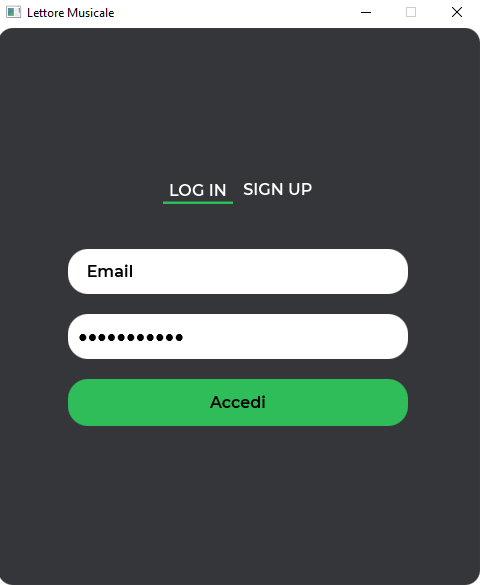
\includegraphics[width=50mm]{schermataLogin.png}} 
		\subfigure[SignIn]{\label{fig:b}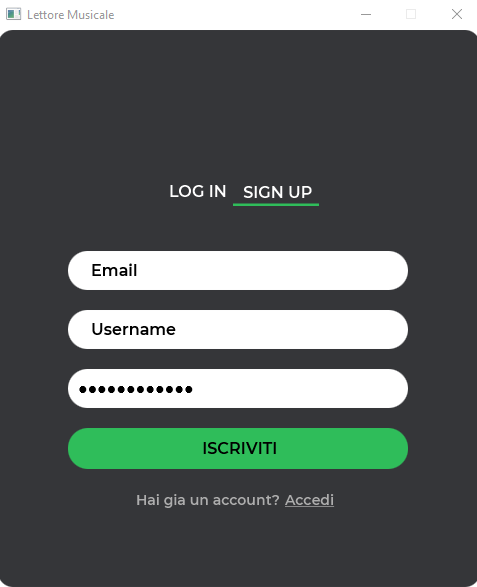
\includegraphics[width=50mm]{schermataLogin_Signin.png}}
		
	\end{figure}
	L'avvenuto successo della registrazione o l'accesso all'applicativo verrà notificato con un \textbf{Allert}, vale anche il l'opposto.
	\begin{figure}[h]
		\centering
		\subfigure[Success]{\label{fig:c}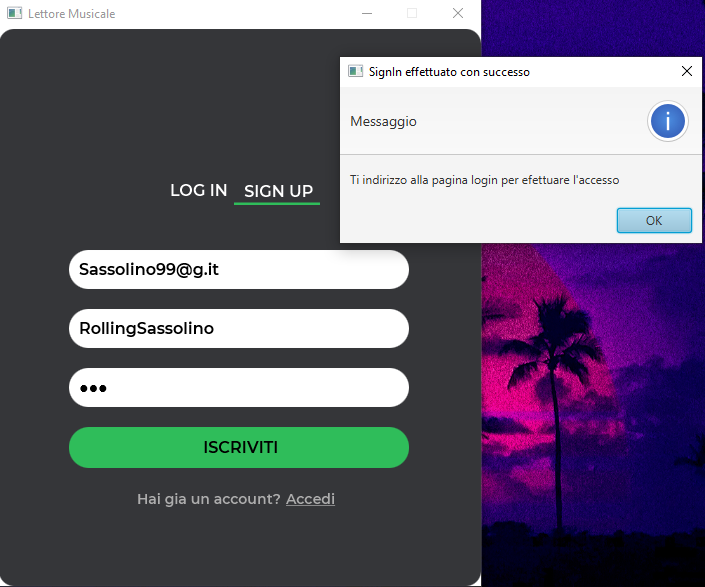
\includegraphics[width=60mm,height=60mm]{succes.png}} 
		\subfigure[Failed]{\label{fig:d}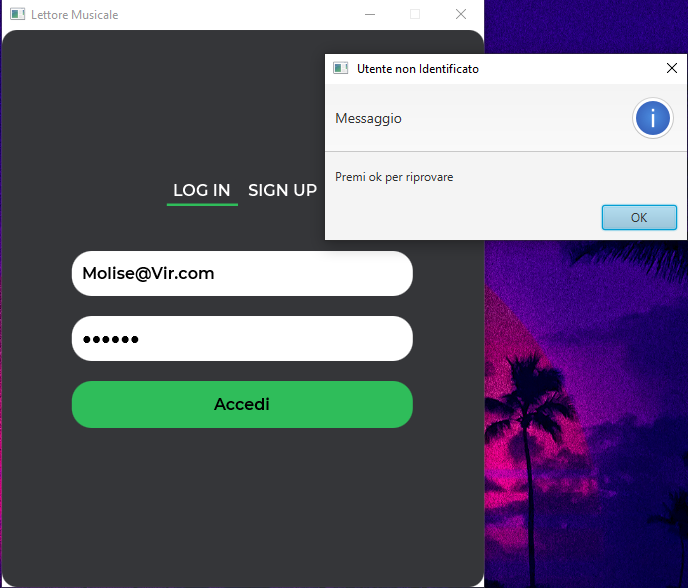
\includegraphics[width=60mm,height=60mm]{failed.png}}
		
	\end{figure}
	\clearpage
	\subsection{Schermata Home}

	Nella schermata \textbf{Home} vengono visualizzate tutte le tracce e utenti prensenti nel database se si clicca su una traccia
	essa verrà segnalata come traccia ascoltata (figura f) e sarà possibile andare nella schermata \textbf{ProfiloAscoltatore} tramite
	l'hyperlink \textbf{"NomeArtista"} se si vuole fare un ricerca personalizzata delle tracce che fanno parte di un album bisogna cliccare
	sul hyperlink  \textbf{"NomeCanzone"} (figura g).
	\begin{figure}[h]
		\centering
		\subfigure[Schermata Home]{\label{fig:a}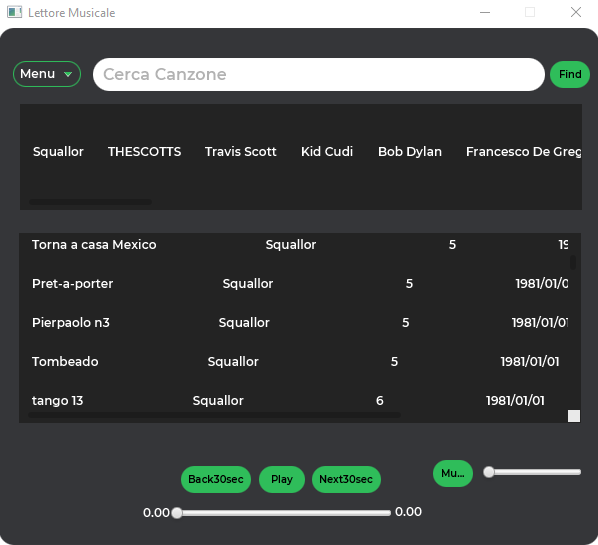
\includegraphics[width=60mm,height=60mm]{SchermataHome.png}} 
		\subfigure[Click Traccia Lista]{\label{fig:b}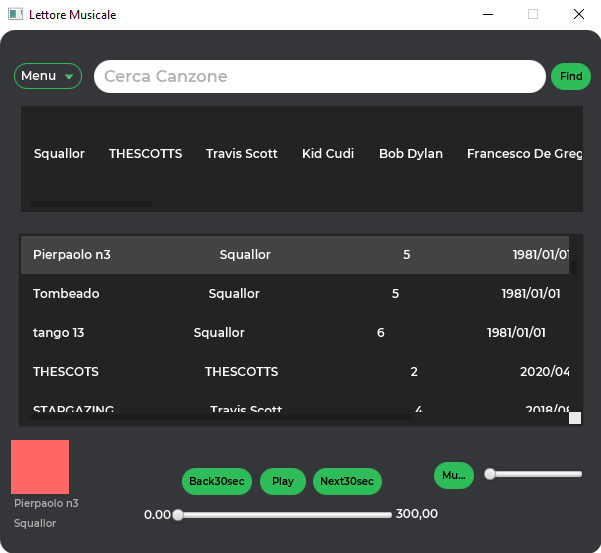
\includegraphics[width=60mm,height=60mm]{SchermataHomeClickSong.png}}
		
	\end{figure}
	Inoltre è possibile fare una ricerca personalizzata (figura h) di utenti e tracce nella barra di ricerca esuccessivamente premendo il tasto \textbf{Find}
	se si preme il tasto find senza con una ricerca vuota verranno visualizzate tutte le tracce e gli utenti presenti nel database.
	\begin{figure}[h]
		\centering
		\subfigure[Click Nome Traccia Link]{\label{fig:a}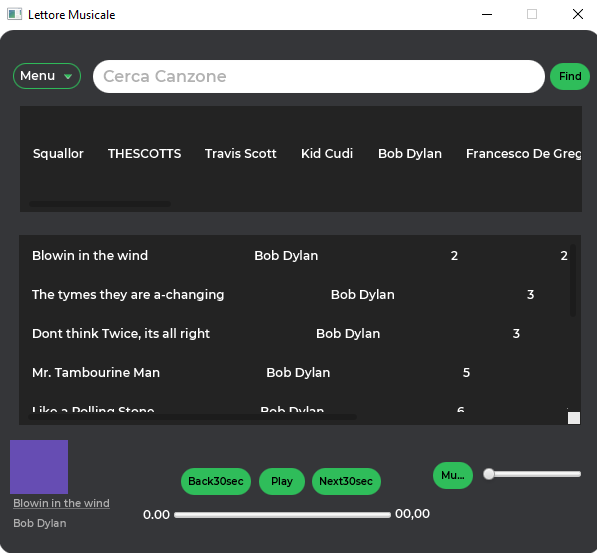
\includegraphics[width=60mm,height=60mm]{SchermataHomeClickLinkTraccia.png}} 
		\subfigure[Ricerca Personalizzata]{\label{fig:b}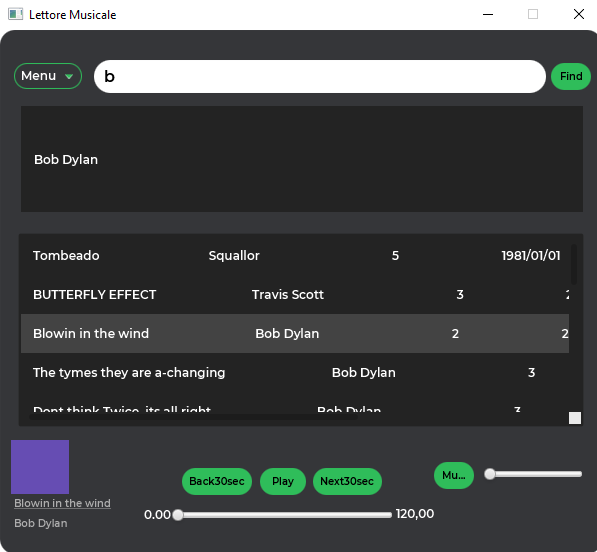
\includegraphics[width=60mm,height=60mm]{SchermataHomeRicercaPersonalizzata.png}}
	\end{figure}
	Nella sezione posta in alto a sinistra è possibile andare nella schermata \textbf{Profilo Personale}, \textbf{Account} e \textbf{Uscire} dall'applicativo.

	\clearpage
	\subsection{Schermata Account}

	Nella schermata \textbf{Account} è presente un form per la modifica di informazioni personali, la prima parte è possibile modificare le info singolarmente 
	invece nella seconda è importante sapere che bisogna dover compilare tutti i campi prima della modifica delle info quali Nome,cognome, BirthDate e tipo Account. 
	Se l'utente è un \textbf{Ascoltatore} avrà la possibilità di modificare solo le sue info (figura e).
	Se l'utente è un \textbf{Artista} allora avrà la possibilità di cambiare schermata (figura f) e poter inserire un nuovo album prodotto nella nuova schermata .
	
	
	\begin{figure}[h]
		\centering
		\subfigure[Account Ascoltatore]{\label{fig:a}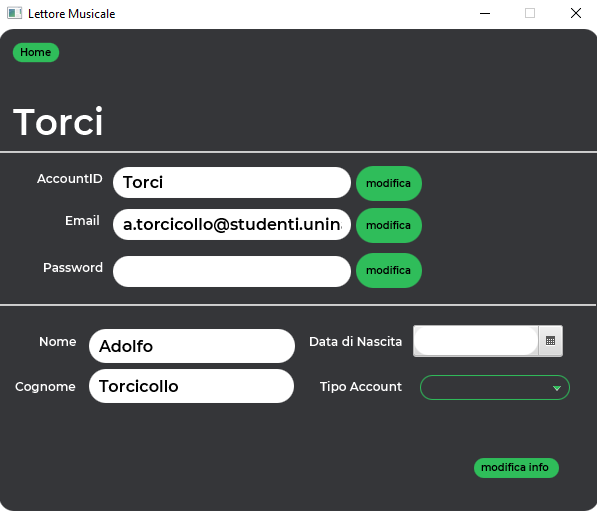
\includegraphics[width=70mm,height=70mm]{Account.png}} 
		\subfigure[Account Artista]{\label{fig:b}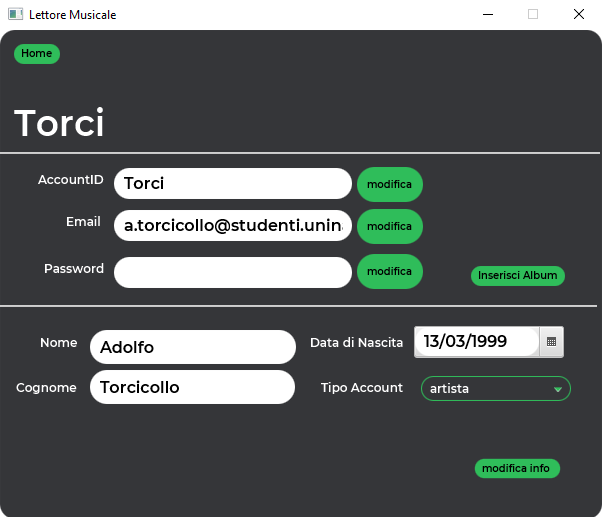
\includegraphics[width=70mm,height=70mm]{AccountArtista.png}}
		
	\end{figure}
	Inoltre è importante sapere che se si vuole cambiare password bisogna sapere la vecchia perchè è richiesta per inserimento di una nuova (figura g).
	\begin{figure}
		\centering
		\subfigure[Modifica Password]{\label{fig:g}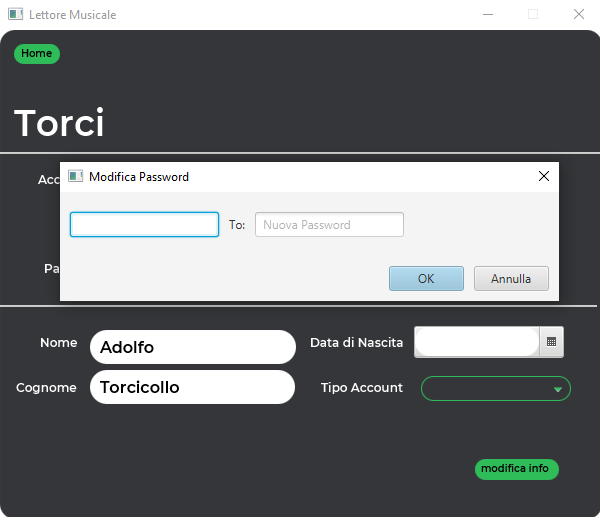
\includegraphics[width=70mm,height=60mm]{accountModificaPassword.png}} 
	\end{figure}

	\clearpage
	\subsection{Schermata InsertMusic}

	Nella schermata \textbf{InserMusic} è presente un form per l'inserimento di un album con le eventuali tracce. I Pulsanti inserisci album e Inserisci Canzone controllano se nel database
	è gia presente tale album o traccia, inoltre non è possibile inserire tracce senza aver prima inserito un album. Il pulsante concludi Inserisce l'album con le eventuali tracce nel Database
	successivamente l'applicativo notificherà l'utente dell'avvenuto caricamento tramite \textbf{Allert} e lo indirizzerà alla schermata home. le seguenti immagini fanno da esempio.
	\begin{figure}[h]
		\centering
		\subfigure[Schermata Vuota]{\label{fig:a}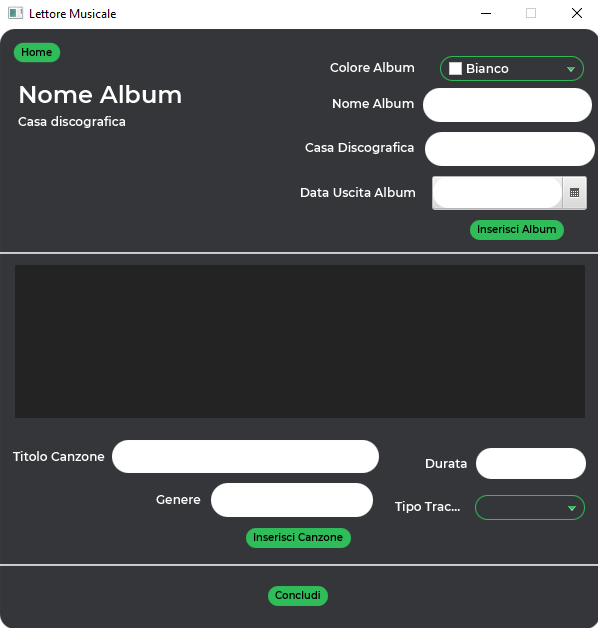
\includegraphics[width=70mm,height=70mm]{InsertMusci.png}} 
		\subfigure[Schermata Dopo aver compilato il form]{\label{fig:b}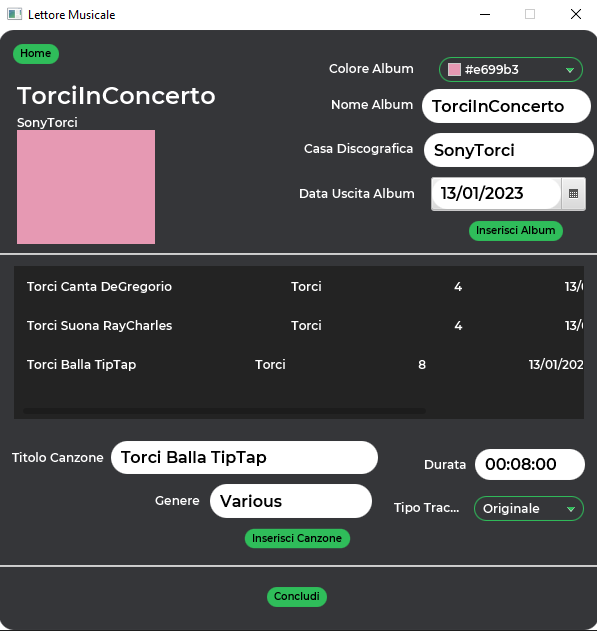
\includegraphics[width=70mm,height=70mm]{InsertMusicInserted.png}}
	\end{figure}

	Inoltre si potranno ascoltare le tracce appena inserito subito dopo (figura a).
	\begin{figure}[h]
		\centering
		\subfigure[Schermata Home dopo L'inserimento]{\label{fig:a}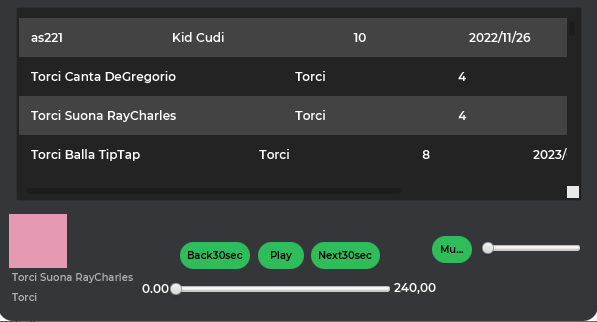
\includegraphics[width=90mm,height=70mm]{InsertMusicResult.png}} 
	\end{figure}

	\clearpage
	\subsection{Schermata ProfiloPersonale o Ascoltatore}

	Nella schermata \textbf{ProfiloAscoltatore} sono presenti le informazioni riguardanti i gusti dell'utente selezionato e come vedremo nel \textbf{ProfiloArtista} se l'utente selezionato non è 
	l'utente loggato esso potrà seguirlo o togliergli il seguito.
	\begin{figure}[h]
		\centering
		\subfigure[Schermata Vuota]{\label{fig:a}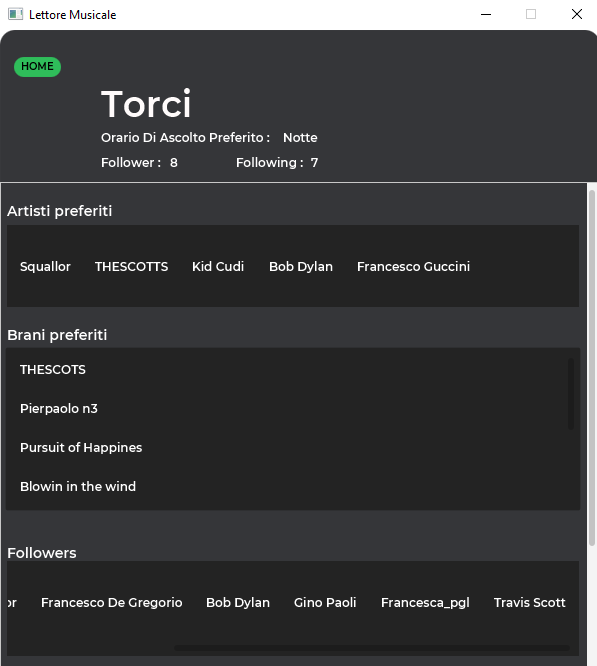
\includegraphics[width=60mm,height=60mm]{ProfiloPersonale1.png}} 
		\subfigure[Schermata Dopo aver compilato il form]{\label{fig:b}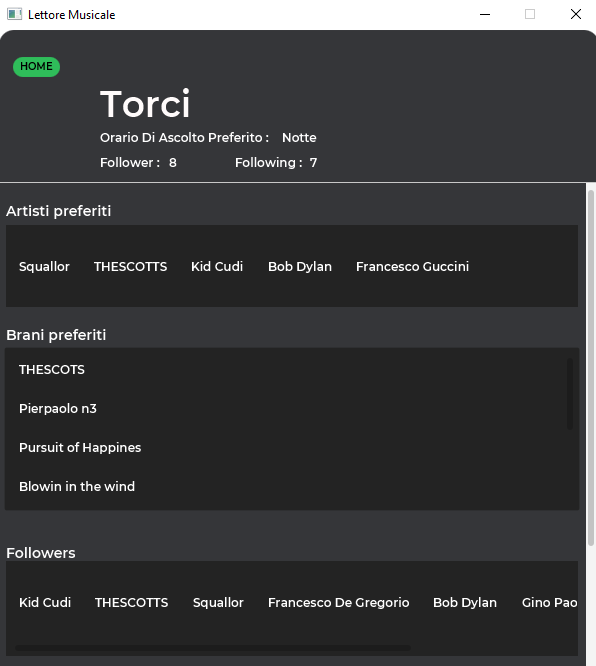
\includegraphics[width=60mm,height=60mm]{ProfiloPersonale2.png}}
	\end{figure}

	\subsection{Schermata ProfiloArtista}

	Nella schermata \textbf{ProfiloArtista} molto simile a quella dell'ascoltatore ma ben differente sotto alcuni aspetti, qui oltre ad essere presenti i nomi dei Followers e Following (presenti anche nel profilo Ascoltatore) 
	sono presenti le informazioni riguardanti l'artista stesso come la discografia e le canzoni popolari.
	Come si è già detto qui è presente il bottone Follow che permette di seguire l'artista oppure togliere il segui. 
	\begin{figure}[h]
		\centering
		\subfigure[Schermata Vuota]{\label{fig:a}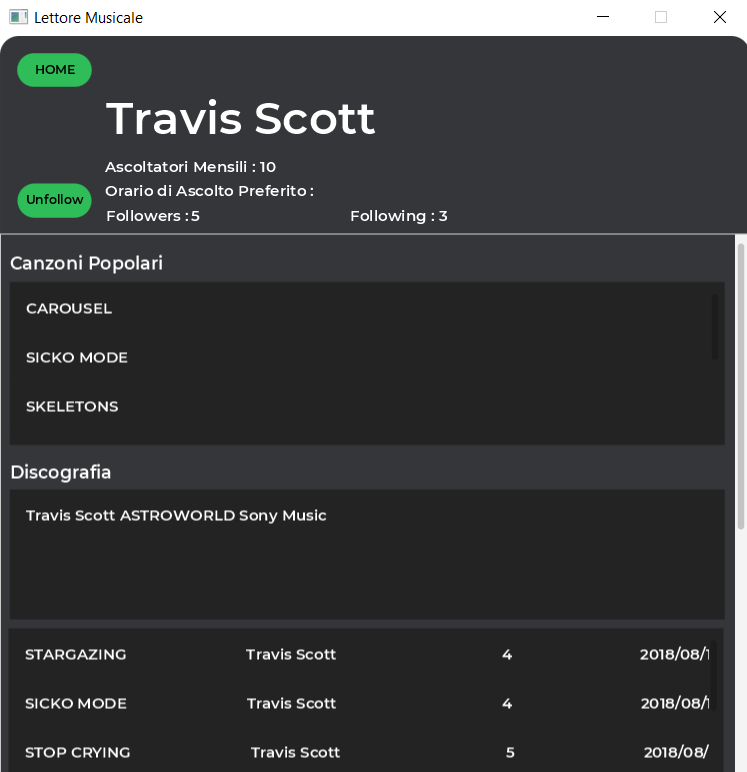
\includegraphics[width=60mm,height=60mm]{ProfiloArtista.png}} 
		\subfigure[Schermata Dopo aver compilato il form]{\label{fig:b}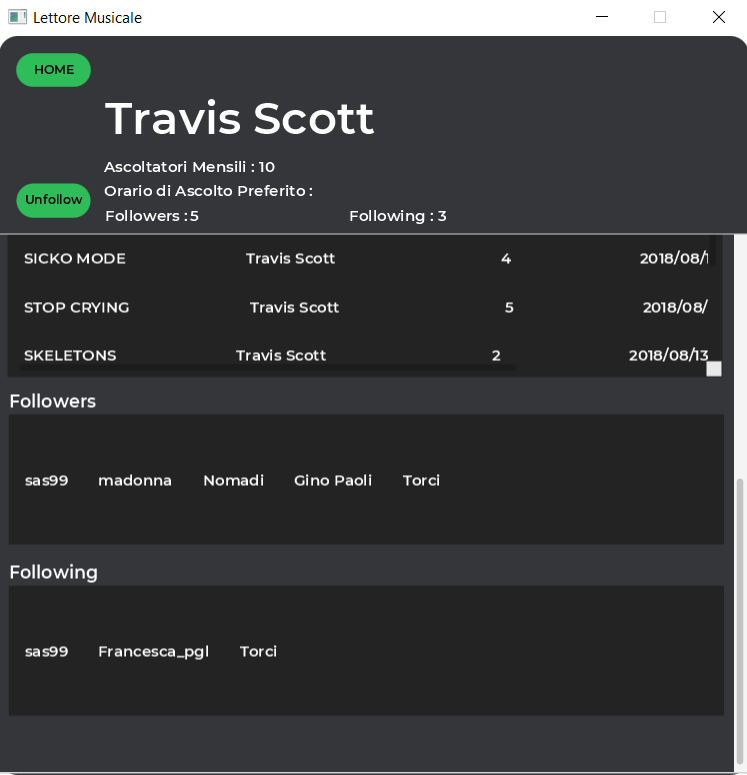
\includegraphics[width=60mm,height=60mm]{ProfiloArtista1.png}}
	\end{figure}

	\end{document}